% ------------------------------------------------------------------------
% ------------------------------------------------------------------------
% abnTeX2: Modelo simples de trabalho acadêmico
% ------------------------------------------------------------------------
% ------------------------------------------------------------------------
 
\documentclass[
	% -- opções da classe memoir --
	12pt,				% tamanho da fonte
	openright,			% capítulos começam em pág ímpar (insere página vazia caso preciso)
	oneside,			% para impressão em recto e verso. Oposto a oneside
	a4paper,			% tamanho do papel. 
	% -- opções da classe abntex2 --
	%chapter=TITLE,		% títulos de capítulos convertidos em letras maiúsculas
	%section=TITLE,		% títulos de seções convertidos em letras maiúsculas
	%subsection=TITLE,	% títulos de subseções convertidos em letras maiúsculas
	%subsubsection=TITLE,% títulos de subsubseções convertidos em letras maiúsculas
	% -- opções do pacote babel --
	english,			% idioma adicional para hifenização
	french,				% idioma adicional para hifenização
	spanish,			% idioma adicional para hifenização
	brazil,				% o último idioma é o principal do documento
	]{abntex2}
 
 
% ---
% PACOTES
% ---

% ---
% Pacotes fundamentais
% ---
\usepackage{lmodern}			% Usa a fonte Latin Modern			
\usepackage[T1]{fontenc}		% Selecao de codigos de fonte.
\usepackage[utf8]{inputenc}		% Codificacao do documento (conversão automática dos acentos)
\usepackage{indentfirst}		% Indenta o primeiro parágrafo de cada seção.
\usepackage{color}				% Controle das cores
\usepackage{graphicx}			% Inclusão de gráficos
\usepackage{microtype} 			% para melhorias de justificação
\usepackage{booktabs} % Para \toprule, \midrule, \bottomrule
\usepackage[table]{xcolor} % Para colorir tabelas

% ---
% Pacotes de citações
% ---
% \usepackage[brazilian,hyperpageref]{backref}	 % Paginas com as citações na bibl
% \usepackage[alf]{abntex2cite}	% Citações padrão ABNT
% ---

% ---
% Informações de dados para CAPA e FOLHA DE ROSTO
% ---
\instituicao{%
  PONTIFÍCIA UNIVERSIDADE CATÓLICA DE MINAS GERAIS
  \par
  PUC Minas Virtual
}
\titulo{Proposta de Solução para o Sistema VOEBEM}
\autor{Frederyck Baleeiro Espinheiro Sales}
\local{Castanhal - PA}
\data{Abril de 2025}
\preambulo{ATIVIDADE DE NIVELAMENTO}
% ---
 
 
% ---
% Configurações de aparência do PDF final
 
% alterando o aspecto da cor azul
\definecolor{blue}{RGB}{41,5,195}
 
% informações do PDF
\makeatletter
\hypersetup{
     	%pagebackref=true,
		pdftitle={\@title},
		pdfauthor={Equipe \abnTeX}, % Corrigido para usar \abnTeX diretamente
    	pdfsubject={\imprimirpreambulo},
	    pdfcreator={LaTeX with abnTeX2},
		pdfkeywords={abnt}{latex}{abntex}{abntex2},
		colorlinks=true,       		% false: boxed links; true: colored links
    	linkcolor=blue,          	% color of internal links
    	citecolor=blue,        		% color of links to bibliography
    	filecolor=magenta,      		% color of file links
		urlcolor=blue,
		bookmarksdepth=4
}
\makeatother

% ---
 
% ---
% Espaçamentos entre linhas e parágrafos
% ---
 
% O tamanho do parágrafo é dado por:
\setlength{\parindent}{1.3cm}
 
% Controle do espaçamento entre um parágrafo e outro:
\setlength{\parskip}{0.2cm}  % tente também \onelineskip
% ---

% ---
% compila o indice
% ---
% \makeindex
% ---
 
% ----
% Início do documento
% ----
\begin{document}
 
% Retira espaço extra obsoleto entre as frases.
\frenchspacing
 
% ----------------------------------------------------------
% ELEMENTOS PRÉ-TEXTUAIS
% ----------------------------------------------------------
 
% ---
% Capa
% ---
\imprimircapa% Garantido sem espaço
% ---
 
% ---
% inserir o sumario
% ---
\pdfbookmark[0]{\contentsname}{toc}
\tableofcontents*
\cleardoublepage% Garantido sem espaço
% ---
  
 
% ----------------------------------------------------------
% ELEMENTOS TEXTUAIS
% ----------------------------------------------------------
\textual% Garantido sem espaço
 % ----------------------------------------------------------
% Inclusão dos Capítulos
% ----------------------------------------------------------


% ----------------------------------------------------------
% Capítulo 1
% ----------------------------------------------------------
% ----------------------------------------------------------
% Capítulo 1
% ----------------------------------------------------------
\chapter{Arquitetura do Sistema - Diagrama C4}
\label{chap:arquitetura-c4}

Para ilustrar claramente a arquitetura proposta para o Sistema VOEBEM, utilizamos a metodologia C4 Model. Esta abordagem fornece diferentes níveis de detalhe, desde uma visão geral do contexto até a estrutura interna dos componentes principais, facilitando a compreensão por diferentes públicos (técnicos e de negócio).

\section{Nível 1 (Contexto)}
\label{sec:c4-contexto}

Este diagrama mostra o Sistema de Reservas VOEBEM em seu contexto, identificando os principais usuários e as integrações com sistemas externos essenciais para sua operação.

\begin{figure}[htbp]
    \centering
    % Nota: A compilação de SVG pode exigir pacotes adicionais como 'svg'.
    % Considere converter as imagens para PDF ou pdf para compatibilidade padrão com pdflatex.
    % Alterado de .pdf para .pdf
    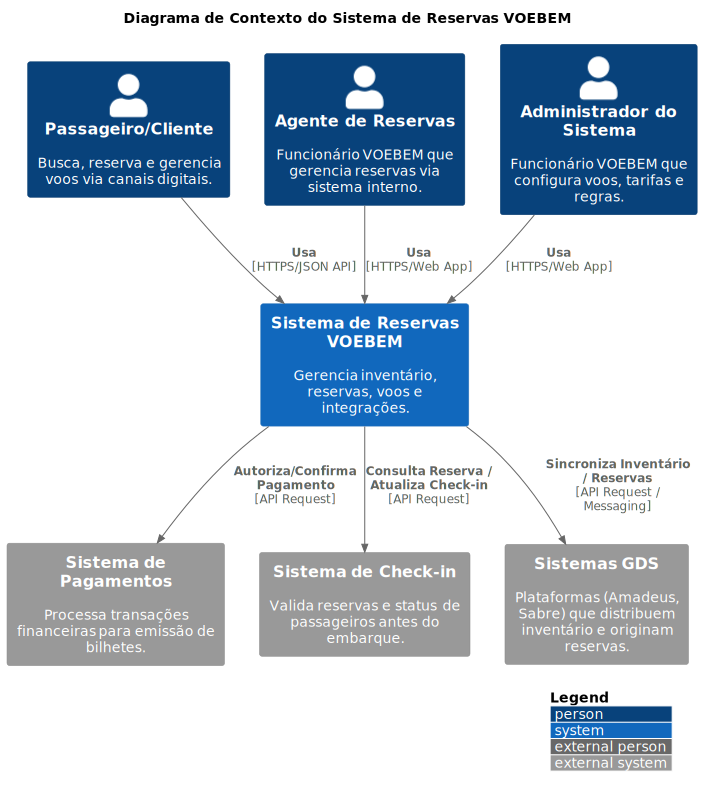
\includegraphics[width=0.9\textwidth]{../assets/c4-n1-contexto.pdf}
    \caption{Diagrama de Contexto C4 - Sistema VOEBEM}
    \label{fig:c4-contexto}
\end{figure}

\subsection{Usuários (Personas)}
\label{subsec:c4-contexto-usuarios}
\begin{itemize}
    \item \textbf{Passageiro/Cliente:} Pessoa que busca, reserva e gerencia voos através dos canais digitais (Website/App Mobile).
    \item \textbf{Agente de Reservas (Funcionário VOEBEM):} Funcionário que utiliza o sistema internamente para criar, modificar e gerenciar reservas em nome dos clientes.
    \item \textbf{Administrador do Sistema (Funcionário VOEBEM):} Funcionário responsável pela configuração de voos, tarifas, regras de negócio e gerenciamento geral do sistema.
\end{itemize}

\subsection{Sistema Principal}
\label{subsec:c4-contexto-sistema-principal}
\begin{itemize}
    \item \textbf{Sistema de Reservas VOEBEM (Software System):} A aplicação central que gerencia todo o inventário de voos, trechos, assentos, processa reservas e fornece informações aos usuários e sistemas externos.
\end{itemize}

\subsection{Sistemas Externos}
\label{subsec:c4-contexto-sistemas-externos}
\begin{itemize}
    \item \textbf{Sistema de Pagamentos (External System):} Serviço externo responsável pelo processamento seguro de transações financeiras para a emissão de bilhetes. \textit{Interage com o Sistema VOEBEM para autorizar e confirmar pagamentos.}
    \item \textbf{Sistema de Check-in (External System):} Sistema utilizado nos aeroportos (ou online) para validar reservas, confirmar a presença do passageiro e atribuir/confirmar assentos antes do embarque. \textit{Interage com o Sistema VOEBEM para consultar dados da reserva/assento e atualizar o status de check-in.}
    \item \textbf{Sistemas GDS (Global Distribution Systems) (External System):} Plataformas globais (Exemplo: Amadeus, Sabre) que distribuem o inventário de voos da VOEBEM para agências de viagens e outros canais. \textit{Interage com o Sistema VOEBEM para consultar disponibilidade, criar reservas (originadas externamente) e sincronizar informações.}
\end{itemize}

\section{Nível 2 (Container)}
\label{sec:c4-container}

Este diagrama detalha os principais blocos de construção (containers) do Sistema de Reservas VOEBEM, suas responsabilidades, tecnologias e como eles interagem, utilizando um banco de dados centralizado conforme requisito.

\begin{figure}[htbp]
    \centering
    % Alterado de .pdf para .pdf
    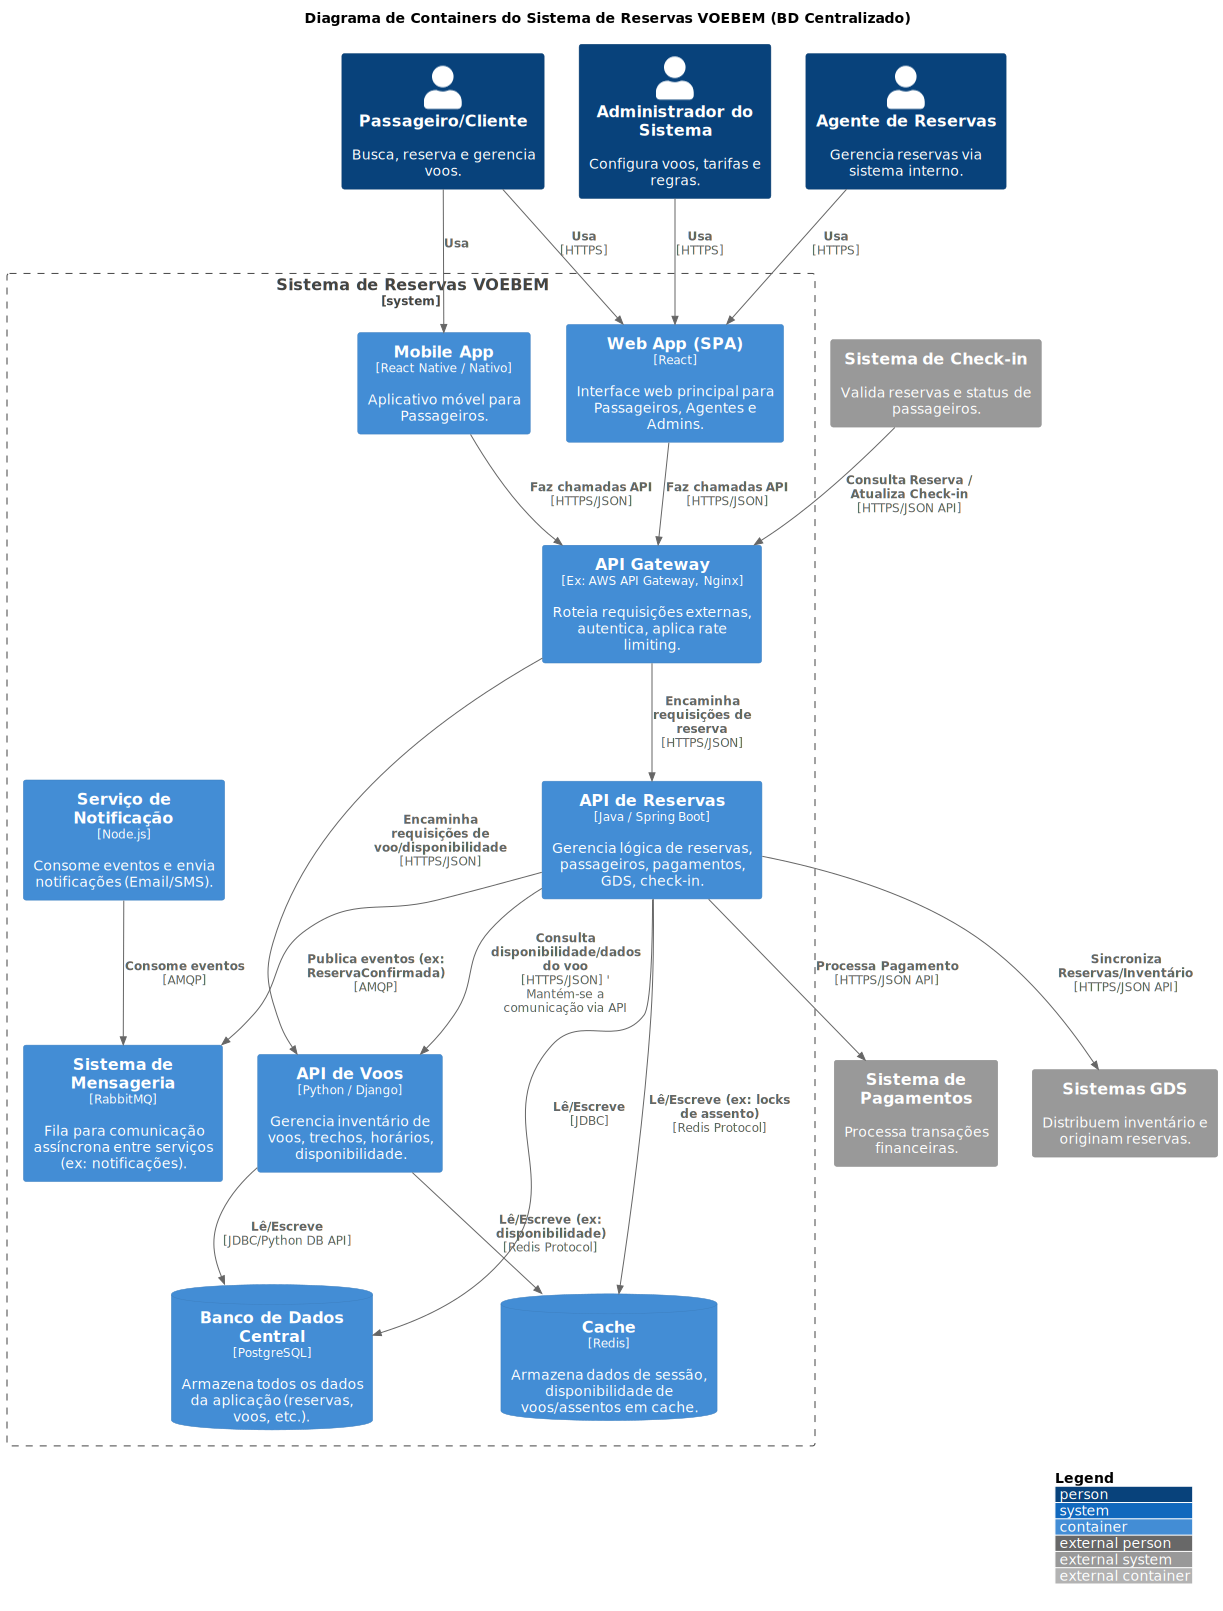
\includegraphics[width=0.9\textwidth]{../assets/c4-n2-container.pdf}
    \caption{Diagrama de Containers C4 - Sistema VOEBEM}
    \label{fig:c4-container}
\end{figure}

\subsection{Containers Principais}
\label{subsec:c4-container-principais}

\textbf{Web App (SPA) (Container)}
\begin{itemize}
    \item \textbf{Descrição:} Interface web principal acessada via navegador.
    \item \textbf{Tecnologia:} React.
    \item \textbf{Responsabilidade:} Fornecer a interface do usuário para Passageiros, Agentes de Reservas e Administradores realizarem suas tarefas (consultas, reservas, gerenciamento).
    \item \textbf{Interage com:} API Gateway (via HTTPS/JSON).
\end{itemize}

\textbf{Mobile App (Container)}
\begin{itemize}
    \item \textbf{Descrição:} Aplicativo móvel nativo ou híbrido.
    \item \textbf{Tecnologia:} React Native / Nativo (iOS/Android).
    \item \textbf{Responsabilidade:} Fornecer uma interface otimizada para Passageiros em dispositivos móveis.
    \item \textbf{Interage com:} API Gateway (via HTTPS/JSON).
\end{itemize}

\textbf{API Gateway (Container)}
\begin{itemize}
    \item \textbf{Descrição:} Ponto único de entrada para todas as requisições externas das interfaces (SPA, Mobile App) e de sistemas externos (Check-in).
    \item \textbf{Tecnologia:} Exemplo: AWS API Gateway, Nginx, Kong.
    \item \textbf{Responsabilidade:} Roteamento de requisições para os serviços backend apropriados, autenticação/autorização inicial, aplicação de rate limiting, agregação leve de respostas (opcional).
    \item \textbf{Interage com:} Web App, Mobile App, Sistema de Check-in, API de Reservas, API de Voos.
\end{itemize}

\textbf{API de Reservas (Container)}
\begin{itemize}
    \item \textbf{Descrição:} Microsserviço backend focado no domínio de reservas.
    \item \textbf{Tecnologia:} Java / Spring Boot.
    \item \textbf{Responsabilidade:} Gerenciar todo o ciclo de vida das reservas (criação, consulta, cancelamento, prorrogação), dados de passageiros, orquestrar interações com pagamento, GDS e check-in, gerenciar reserva de assentos.
    \item \textbf{Interage com:} API Gateway, Banco de Dados Central, API de Voos, Cache, Sistema de Mensageria, Sistema de Pagamentos, Sistemas GDS.
\end{itemize}

\textbf{API de Voos (Container)}
\begin{itemize}
    \item \textbf{Descrição:} Microsserviço backend focado no domínio de inventário de voos.
    \item \textbf{Tecnologia:} Python / Django.
    \item \textbf{Responsabilidade:} Gerenciar informações sobre voos, trechos, horários, aeroportos, aeronaves e calcular/consultar disponibilidade de voos e assentos.
    \item \textbf{Interage com:} API Gateway, Banco de Dados Central, Cache, API de Reservas.
\end{itemize}

\textbf{Serviço de Notificação (Container)}
\begin{itemize}
    \item \textbf{Descrição:} Serviço assíncrono para envio de notificações.
    \item \textbf{Tecnologia:} Node.js.
    \item \textbf{Responsabilidade:} Consumir eventos do Sistema de Mensageria (Exemplo: \texttt{ReservaConfirmada}, \texttt{PrazoExpirando}) e enviar notificações aos usuários via canais apropriados (Email, SMS - integração com serviços externos específicos não mostrada neste nível).
    \item \textbf{Interage com:} Sistema de Mensageria.
\end{itemize}

\subsection{Containers de Dados e Mensageria}
\label{subsec:c4-container-dados}

\textbf{Banco de Dados Central (Database Container)}
\begin{itemize}
    \item \textbf{Descrição:} Banco de dados relacional centralizado que armazena todos os dados da aplicação.
    \item \textbf{Tecnologia:} PostgreSQL.
    \item \textbf{Responsabilidade:} Armazenar de forma persistente e transacional os dados de reservas, passageiros, voos, trechos, aeroportos, aeronaves, assentos, etc.
    \item \textbf{Acessado por:} API de Reservas, API de Voos.
\end{itemize}

\textbf{Cache (Database Container)}
\begin{itemize}
    \item \textbf{Descrição:} Armazenamento de dados em memória para acesso rápido.
    \item \textbf{Tecnologia:} Redis.
    \item \item \textbf{Responsabilidade:} Acelerar consultas frequentes (Exemplo: disponibilidade de voos/assentos), armazenar dados de sessão (opcional), gerenciar locks temporários (Exemplo: durante seleção de assento).
    \item \textbf{Acessado por:} API de Reservas, API de Voos.
\end{itemize}

\textbf{Sistema de Mensageria (Container)}
\begin{itemize}
    \item \textbf{Descrição:} Broker de mensagens para comunicação assíncrona.
    \item \textbf{Tecnologia:} RabbitMQ.
    \item \textbf{Responsabilidade:} Desacoplar a comunicação entre serviços, permitindo que eventos sejam publicados (pela API de Reservas) e consumidos (pelo Serviço de Notificação) de forma independente e resiliente.
    \item \textbf{Acessado por:} API de Reservas, Serviço de Notificação.
\end{itemize}

\section{Nível 3 (Componentes - Exemplo para API de Reservas)}
\label{sec:c4-componentes}

Este diagrama detalha a estrutura interna do container "API de Reservas", mostrando seus principais componentes lógicos e como eles colaboram para realizar as funcionalidades de reserva e interagir com dependências externas.

\begin{figure}[htbp]
    \centering
    % Adicionando angle=90 para rotacionar a imagem
    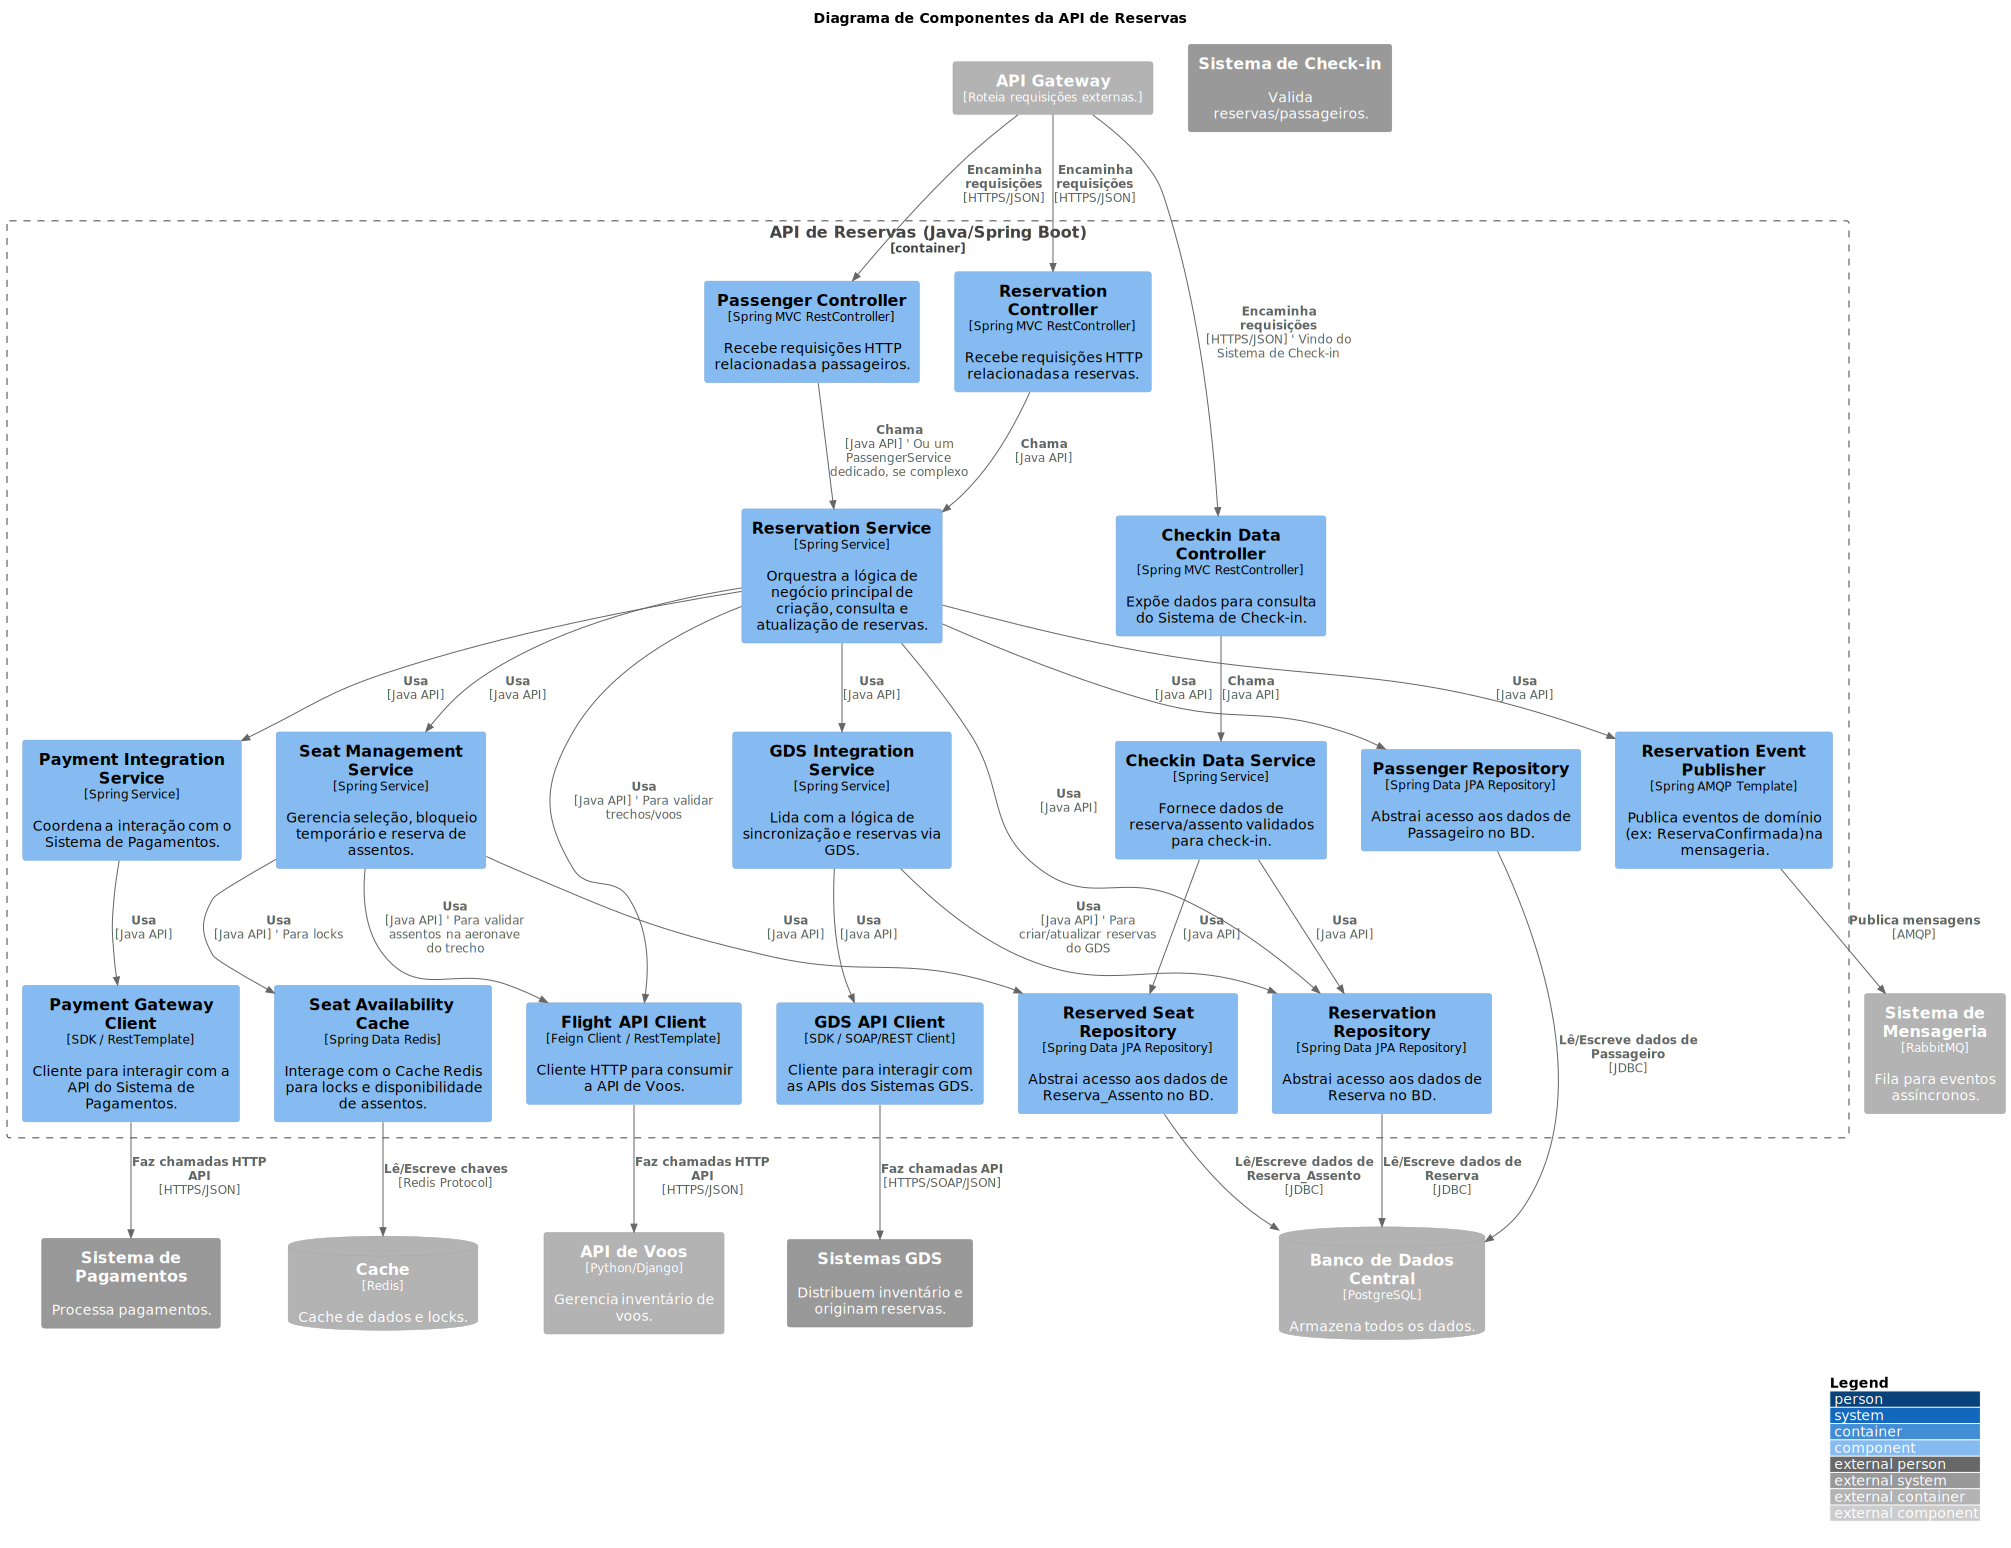
\includegraphics[width=1.4\textwidth, angle=90]{../assets/c4-n3-component-api-reservas.pdf}
    \caption{Diagrama de Componentes C4 - API de Reservas}
    \label{fig:c4-componentes-api-reservas}
\end{figure}

\subsection{Componentes Principais da API de Reservas}
\label{subsec:c4-componentes-api-reservas-principais}

\textbf{Controllers (\texttt{ReservationController}, \texttt{PassengerController}, \texttt{CheckinDataController})}
\begin{itemize}
    \item \textbf{Tecnologia:} Spring MVC RestController.
    \item \textbf{Responsabilidade:} Receber requisições HTTP da API Gateway, validar entradas básicas e delegar para os serviços apropriados. O \texttt{CheckinDataController} expõe endpoints específicos para consulta pelo Sistema de Check-in.
\end{itemize}

\textbf{Services (\texttt{ReservationService}, \texttt{SeatManagementService}, \texttt{PaymentIntegrationService}, \texttt{GdsIntegrationService}, \texttt{CheckinDataService})}
\begin{itemize}
    \item \textbf{Tecnologia:} Spring Service.
    \item \textbf{Responsabilidade:} Contêm a lógica de negócio principal.
    \begin{itemize}
        \item \texttt{ReservationService}: Orquestra o fluxo de criação, consulta, atualização de reservas, validações de regras de negócio.
        \item \texttt{SeatManagementService}: Gerencia a lógica de seleção, bloqueio temporário (usando cache) e confirmação de assentos.
        \item \texttt{PaymentIntegrationService}: Coordena a comunicação com o \texttt{PaymentGatewayClient} para processar pagamentos.
        \item \texttt{GdsIntegrationService}: Lida com a lógica de receber/enviar dados de/para os \texttt{Sistemas GDS} através do \texttt{GdsApiClient}.
        \item \texttt{CheckinDataService}: Fornece dados consolidados e validados sobre a reserva e assento para o \texttt{CheckinDataController}.
    \end{itemize}
\end{itemize}

\textbf{Repositories (\texttt{ReservationRepository}, \texttt{PassengerRepository}, \texttt{ReservedSeatRepository})}
\begin{itemize}
    \item \textbf{Tecnologia:} Spring Data JPA Repository.
    \item \textbf{Responsabilidade:} Abstrair o acesso (leitura/escrita) aos dados das entidades correspondentes no \texttt{Banco de Dados Central}.
\end{itemize}

\textbf{Clients (\texttt{FlightApiClient}, \texttt{PaymentGatewayClient}, \texttt{GdsApiClient})}
\begin{itemize}
    \item \textbf{Tecnologia:} Feign Client / RestTemplate / SDKs específicos.
    \item \textbf{Responsabilidade:} Encapsular a comunicação via rede com outros containers ou sistemas externos.
    \begin{itemize}
        \item \texttt{FlightApiClient}: Comunica-se com a \texttt{API de Voos} para obter informações de voos, trechos e validar disponibilidade/assentos.
        \item \texttt{PaymentGatewayClient}: Interage com o \texttt{Sistema de Pagamentos} externo.
        \item \texttt{GdsApiClient}: Interage com os \texttt{Sistemas GDS} externos.
    \end{itemize}
\end{itemize}

\textbf{Messaging (\texttt{ReservationEventPublisher})}
\begin{itemize}
    \item \textbf{Tecnologia:} Spring AMQP Template.
    \item \textbf{Responsabilidade:} Publicar eventos de domínio significativos (Exemplo: \texttt{ReservaConfirmada}, \texttt{PagamentoFalhou}) no \texttt{Sistema de Mensageria} para processamento assíncrono (Exemplo: notificações).
\end{itemize}

\textbf{Caching (\texttt{SeatAvailabilityCache})}
\begin{itemize}
    \item \textbf{Tecnologia:} Spring Data Redis.
    \item \textbf{Responsabilidade:} Interagir com o \texttt{Cache (Redis)} para operações específicas, como gerenciamento de locks distribuídos durante a seleção de assentos para evitar concorrência.
\end{itemize}

\section{Destaques Obrigatórios}
\label{sec:destaques-obrigatorios}

\subsection{Escalabilidade}
\label{subsec:escalabilidade}
\begin{itemize}
    \item \textbf{Horizontal:} Utilização de múltiplos containers/instâncias para os serviços (Frontend, API Gateway, Serviços Backend) gerenciados por orquestradores (Kubernetes, AWS ECS) ou grupos de autoescalonamento (Auto Scaling Groups). O Banco de Dados pode escalar leituras com réplicas.
    \item \textbf{Vertical:} Aumento de recursos (CPU/Memória) das instâncias/containers conforme necessário (menos preferível para serviços stateless).
\end{itemize}

\subsection{Balanceamento de Carga}
\label{subsec:balanceamento-carga}
Uso de Load Balancers (Exemplo: AWS ELB, Nginx) na frente da API Gateway e dos serviços backend para distribuir o tráfego entre as instâncias disponíveis.

\subsection{Alta Disponibilidade}
\label{subsec:alta-disponibilidade}
\begin{itemize}
    \item Deploy das instâncias/containers em múltiplas Zonas de Disponibilidade (AZs) na nuvem.
    \item Uso de bancos de dados gerenciados com replicação multi-AZ e failover automático.
    \item Implementação de Health Checks para que o Load Balancer e o orquestrador removam instâncias não saudáveis.
\end{itemize}

% --- Final do Arquivo ---
% ----------------------------------------------------------
% Capítulo 2
% ----------------------------------------------------------
% ----------------------------------------------------------
% Capítulo 2
% ----------------------------------------------------------
\chapter{Estratégia de Deploy e Resiliência}
\label{chap:deploy-resiliencia}

Esta seção detalha as estratégias propostas para garantir entregas de software frequentes, confiáveis e com baixo risco para o Sistema VOEBEM, abordando o pipeline de CI/CD, a metodologia de deploy em produção e o plano de rollback.

\section{Pipeline de CI/CD (Integração Contínua / Entrega Contínua)}
\label{sec:cicd}

Propõe-se um pipeline de CI/CD robusto para automatizar o processo de build, teste e deploy dos diferentes containers (microsserviços, frontend) do sistema, conforme ilustrado abaixo.

\subsection{Ferramentas Propostas}
\label{subsec:cicd-ferramentas}
\begin{itemize}
    \item \textbf{Controle de Versão:} Git (com repositórios hospedados no GitLab ou GitHub).
    \item \textbf{Servidor de CI/CD:} GitLab CI/CD ou GitHub Actions (integrados à plataforma de repositórios).
    \item \textbf{Containerização:} Docker (para empacotar as aplicações e suas dependências).
    \item \textbf{Registro de Container:} Docker Hub, GitLab Container Registry, AWS ECR ou similar.
    \item \textbf{Orquestração de Containers:} Kubernetes (gerenciado na nuvem, Exemplo: AWS EKS, Google GKE, Azure AKS).
    \item \textbf{Ferramentas de Teste:} JUnit (para Java/API Reservas), PyTest (para Python/API Voos), Jest/Cypress (para Frontend React).
    \item \textbf{Análise de Código (Opcional):} SonarQube (para análise estática de segurança e qualidade).
\end{itemize}

\subsection{Fluxo do Pipeline}
\label{subsec:cicd-fluxo}
O diagrama abaixo ilustra as etapas sequenciais e pontos de decisão do pipeline, desde o commit do código até o deploy em produção, incluindo validações intermediárias.

\begin{figure}[htbp]
    \centering
    % Ajustando largura para consistência com Cap. 3
    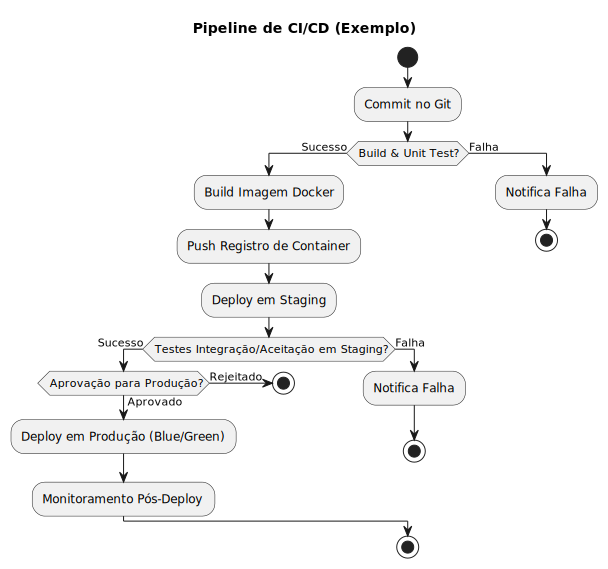
\includegraphics[width=0.8\textwidth]{assets/diagrama-cicd.pdf}
    \caption{Diagrama do Pipeline de CI/CD}
    \label{fig:diagrama-cicd}
\end{figure}

\subsection{Etapas Detalhadas}
\label{subsec:cicd-etapas}
\begin{enumerate}
    \item \textbf{Commit \& Trigger:} Desenvolvedor envia código, iniciando o pipeline.
    \item \textbf{Build \& Unit Test:} Compilação e testes unitários. Falhas interrompem o pipeline.
    \item \textbf{Code Scan (Opcional):} Análise estática de código.
    \item \textbf{Build da Imagem Docker:} Criação da imagem da aplicação.
    \item \textbf{Push para Registro:} Envio da imagem para o registro.
    \item \textbf{Deploy em Staging:} Implantação em ambiente de homologação.
    \item \textbf{Testes de Integração/Aceitação:} Validação funcional e de integração em Staging. Falhas interrompem o pipeline.
    \item \textbf{Aprovação (Manual/Automática):} Ponto de controle antes da produção.
    \item \textbf{Deploy em Produção:} Implantação em produção usando a estratégia Blue/Green.
    \item \textbf{Monitoramento Pós-Deploy:} Observação ativa da nova versão em produção.
\end{enumerate}

\section{Estratégia de Deploy}
\label{sec:estrategia-deploy}

Considerando a criticidade do sistema e a necessidade de minimizar riscos e downtime, a estratégia de deploy recomendada é \textbf{Blue/Green Deployment}, cujo fluxo é apresentado no diagrama a seguir.

\subsection{Justificativa}
\label{subsec:deploy-justificativa}
\begin{itemize}
    \item \textbf{Zero Downtime:} Transição suave de tráfego.
    \item \textbf{Testes em Produção Isolados:} Validação da nova versão sem impacto no usuário.
    \item \textbf{Rollback Instantâneo:} Reversão rápida em caso de problemas.
    \item \textbf{Simplicidade Conceitual:} Fluxo claro para deploy e rollback.
\end{itemize}

\subsection{Funcionamento (Ilustrado no Diagrama)}
\label{subsec:deploy-funcionamento}

\begin{figure}[htbp]
    \centering
    % Ajustando largura para consistência com Cap. 3
    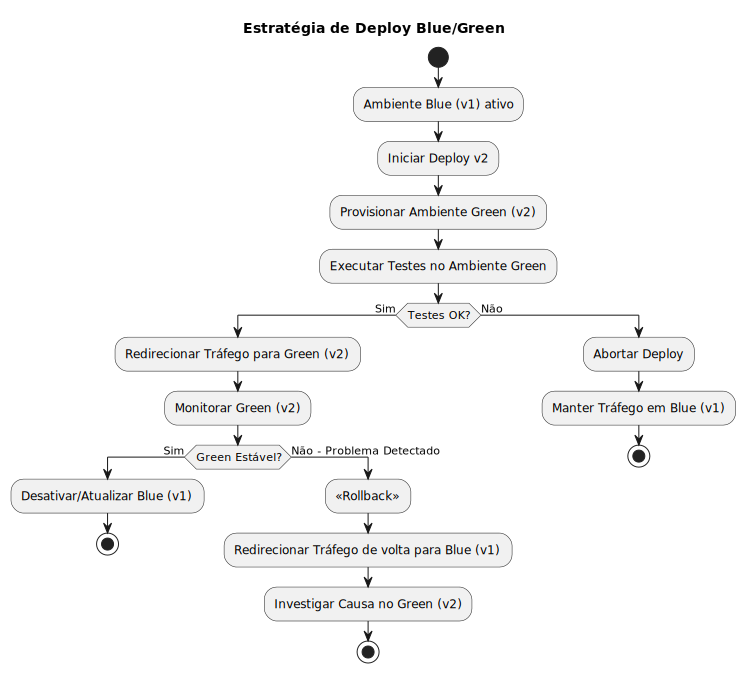
\includegraphics[width=0.8\textwidth]{assets/diagrama-bluegreen.pdf}
    \caption{Diagrama da Estratégia Blue/Green}
    \label{fig:diagrama-bluegreen}
\end{figure}

\begin{enumerate}
    \item \textbf{Ambiente Blue Ativo:} Versão atual (v1) recebe o tráfego.
    \item \textbf{Provisionamento Green:} Nova versão (v2) é implantada em um ambiente idêntico (Green).
    \item \textbf{Testes no Green:} Validação da v2 no ambiente Green isolado.
    \item \textbf{Switch de Tráfego:} Se os testes passarem, o tráfego é direcionado para o ambiente Green (v2).
    \item \textbf{Monitoramento do Green:} A v2 é monitorada em produção.
    \item \textbf{Estabilização ou Rollback:} Se a v2 estiver estável, o ambiente Blue (v1) é desativado. Se problemas críticos forem detectados, o tráfego é revertido imediatamente para o Blue (v1) (Rollback).
    \item \textbf{Desativação do Blue:} Após confirmação da estabilidade do Green, o ambiente Blue é liberado.
\end{enumerate}

\subsection{Benefícios para VOEBEM}
\label{subsec:deploy-beneficios}
Essa abordagem minimiza o risco de impacto ao usuário durante atualizações e permite reversões imediatas caso surjam problemas inesperados, garantindo assim a continuidade das operações críticas de reserva e a confiança do cliente.

\section{Estratégia de Rollback}
\label{sec:estrategia-rollback}

A estratégia de rollback é uma parte intrínseca do fluxo Blue/Green, como visualizado no diagrama anterior.

\subsection{Processo de Rollback (Detalhado)}
\label{subsec:rollback-processo}
\begin{enumerate}
    \item \textbf{Detecção de Problema:} Identificação de falha crítica na versão Green (v2) ativa, via monitoramento ou alertas.
    \item \textbf{Acionamento:} Manual pela equipe SRE/Operações ou automático por violação de SLOs.
    \item \textbf{Redirecionamento de Tráfego:} Reconfiguração do Load Balancer/Roteador para enviar 100% do tráfego de volta ao ambiente Blue (v1), que contém a versão estável anterior. Esta é a ação principal e imediata do rollback.
    \item \textbf{Análise de Causa Raiz:} Investigação do problema no ambiente Green (v2), agora isolado.
    \item \textbf{Correção e Novo Deploy:} Após correção, o ciclo de deploy pode ser reiniciado.
\end{enumerate}

\subsection{Garantias}
\label{subsec:rollback-garantias}
\begin{itemize}
    \item \textbf{Velocidade:} MTTR minimizado pela rapidez do redirecionamento.
    \item \textbf{Segurança:} Versão estável anterior sempre disponível.
    \item \textbf{Consistência:} Processo claro e passível de automação.
\end{itemize}

% --- Final do Arquivo ---

% ----------------------------------------------------------
% Capítulo 3
% ----------------------------------------------------------
% ----------------------------------------------------------
% Capítulo 3
% ----------------------------------------------------------
\chapter{Plano de Melhoria da Confiabilidade e Percepção do Cliente}
\label{chap:confiabilidade-feedback}

A confiabilidade e a percepção positiva do cliente são cruciais para o sucesso do VOEBEM. Este plano descreve as práticas de Engenharia de Confiabilidade de Sites (SRE - Site Reliability Engineering) que propomos para alcançar e manter altos níveis de serviço, alinhando a operação técnica com a experiência do cliente.

\section{Monitoramento e Observabilidade}
\label{sec:monitoramento}

Uma estratégia robusta de monitoramento e observabilidade é fundamental para entender o comportamento do sistema, detectar problemas proativamente e garantir que as metas de negócio sejam atendidas. Propõe-se uma abordagem baseada nos três pilares da observabilidade: métricas, logs e traces.

\subsection{SLIs (Service Level Indicators) Chave}
\label{subsec:slis}
Indicadores quantitativos que medem aspectos específicos do serviço. Exemplos para VOEBEM:

\begin{table}[htbp]
    \centering
    \caption{Exemplos de SLIs para o Sistema VOEBEM}
    \label{tab:slis}
    \rowcolors{2}{gray!10}{white} % Adiciona cores alternadas (requer \usepackage[table]{xcolor})
    % Usar tabularx e booktabs. Remover linhas verticais.
    \begin{tabularx}{\textwidth}{lX} % Removido '|'
        \toprule % Substitui \hline
        \textbf{Categoria} & \textbf{SLI (Indicador)} \\
        \midrule % Substitui \hline
        Disponibilidade & \% de requisições bem-sucedidas (HTTP 2xx/3xx) na API Gateway (endpoints chave) \\
        Disponibilidade & \% de requisições bem-sucedidas nas APIs (Reservas, Voos) \\
        Latência & Tempo de resposta (p95, p99) para busca de voos na API Gateway \\
        Latência & Tempo de resposta (p95) para criação de reserva na API de Reservas \\
        Taxa de Erros & \% de requisições com erro (HTTP 5xx) nas APIs (Gateway, Reservas, Voos) \\
        Taxa de Erros & Taxa de falhas na integração com Sistema de Pagamentos \\
        Taxa de Erros & Taxa de erros na publicação/consumo de mensagens (Sistema de Mensageria) \\
        Saturação & Uso de CPU/Memória dos containers \\
        Saturação & Uso de conexões do banco de dados \\
        Saturação & Profundidade da fila no Sistema de Mensageria \\
        \bottomrule % Substitui \hline
    \end{tabularx}
\end{table}

\subsection{SLOs (Service Level Objectives)}
\label{subsec:slos}
Metas claras e mensuráveis para os SLIs mais críticos, definindo o nível de serviço esperado. Exemplos:

\begin{table}[htbp]
    \centering
    \caption{Exemplos de SLOs para o Sistema VOEBEM}
    \label{tab:slos}
    \rowcolors{2}{gray!10}{white}
    % Usar tabularx e booktabs.
    \begin{tabularx}{\textwidth}{XXl} % Removido '|'
        \toprule
        \textbf{SLI Referente} & \textbf{Exemplo de SLO (Meta)} & \textbf{Janela} \\
        \midrule
        Disponibilidade API Gateway (Busca/Reserva) & >= 99.9\% de requisições bem-sucedidas & Mensal \\
        Latência Busca de Voos (p95) & < 800ms & Contínua \\
        Latência Criação de Reserva (p95) & < 1500ms & Contínua \\
        Taxa de Erros API Reservas (5xx) & < 0.1\% & Mensal \\
        \bottomrule
    \end{tabularx}
    \par\medskip
    \textit{(Nota: Estes são exemplos iniciais e devem ser refinados com base em dados históricos e necessidades de negócio).}
\end{table}

\subsection{Ferramentas Propostas}
\label{subsec:monitoramento-ferramentas}

\begin{table}[htbp]
    \centering
    \caption{Ferramentas Propostas para Monitoramento e Observabilidade}
    \label{tab:monitoramento-ferramentas}
    \rowcolors{2}{gray!10}{white}
    % Usar tabularx e booktabs.
    \begin{tabularx}{\textwidth}{lXX} % Removido '|'
        \toprule
        \textbf{Pilar} & \textbf{Ferramenta(s) Proposta(s)} & \textbf{Principal Responsabilidade} \\
        \midrule
        Métricas & Prometheus + Grafana & Coleta e Visualização de Métricas (SLIs, SLOs, Saúde) \\
        Logs & Fluentd/Bit + Loki + Grafana (ou ELK Stack) & Coleta, Agregação e Consulta de Logs \\
        Tracing & Jaeger + OpenTelemetry + Grafana & Coleta e Visualização de Traces Distribuídos \\
        Alertas & Alertmanager + PagerDuty/Opsgenie & Definição de Regras de Alerta e Notificação On-Call \\
        \bottomrule
    \end{tabularx}
\end{table}

\subsection{Alertas}
\label{subsec:alertas}
\begin{itemize}
    \item Configurados no \textbf{Alertmanager} (parte do ecossistema Prometheus).
    \item Baseados principalmente na \textbf{violação dos SLOs} (Exemplo: taxa de erro acima do limite por X minutos, latência p99 excedendo o objetivo) ou em \textbf{sintomas críticos} (Exemplo: serviço indisponível, erro de acesso ao banco de dados, fila de mensagens crescendo rapidamente, certificados expirando).
    \item Alertas devem ser \textbf{acionáveis}, indicando claramente o problema e o impacto potencial.
    \item Direcionamento para a equipe de plantão (on-call) através de ferramentas como \textbf{PagerDuty} ou \textbf{Opsgenie}, com diferentes níveis de severidade e canais de notificação (Exemplo: chat, telefone).
\end{itemize}

\section{Automação de Recuperação}
\label{sec:automacao-recuperacao}

Para aumentar a resiliência e reduzir a necessidade de intervenção manual em caso de falhas, propõe-se a implementação de mecanismos de recuperação automática, principalmente aproveitando recursos do Kubernetes e serviços gerenciados na nuvem.

\subsection{Auto-Healing (Kubernetes)}
\label{subsec:auto-healing}
\begin{itemize}
    \item \textbf{Liveness Probes:} Verificações periódicas configuradas nos Deployments/StatefulSets. Se um container falhar na verificação (Exemplo: travado, não respondendo a um endpoint \texttt{/healthz}), o Kubelet o reiniciará automaticamente na mesma instância (Node).
    \item \textbf{Readiness Probes:} Verificações que indicam se um container está pronto para receber tráfego (Exemplo: aplicação iniciada, conexões estabelecidas). O Kubernetes só enviará tráfego (via Services) para Pods que estejam "Ready". Se um Pod falhar na Readiness Probe, ele é temporariamente removido do balanceamento de carga até se recuperar.
    \item \textbf{ReplicaSets/Deployments:} Garantem que o número desejado de réplicas de um serviço esteja sempre em execução. Se um Node falhar, os Pods que estavam nele são automaticamente reagendados em outros Nodes saudáveis.
\end{itemize}

\subsection{Auto-Scaling (Kubernetes)}
\label{subsec:auto-scaling}
\begin{itemize}
    \item \textbf{Horizontal Pod Autoscaler (HPA):} Ajusta automaticamente o número de réplicas de um Deployment/StatefulSet com base em métricas observadas, como utilização média de CPU, memória ou métricas customizadas (Exemplo: requisições por segundo, profundidade de fila via KEDA). Isso garante que o sistema tenha capacidade suficiente para lidar com picos de carga e reduza custos em períodos de baixa utilização.
    \item \textbf{Cluster Autoscaler (Provedor de Nuvem):} Adiciona ou remove automaticamente Nós (VMs) ao cluster Kubernetes com base na demanda por recursos (Pods pendentes por falta de CPU/memória).
\end{itemize}

\subsection{Failover Automático (Componentes Stateful)}
\label{subsec:failover-automatico}
\begin{itemize}
    \item \textbf{Banco de Dados Central (PostgreSQL):} Utilizar um serviço de banco de dados gerenciado na nuvem (Exemplo: AWS RDS, Google Cloud SQL, Azure Database for PostgreSQL) configurado em modo \textbf{Multi-AZ (Multi-Availability Zone)}. O provedor de nuvem gerencia a replicação síncrona para uma instância standby em outra AZ e realiza o failover automático para a standby em caso de falha da instância primária, com mínima interrupção.
    \item \textbf{Cache (Redis):} Utilizar um serviço gerenciado (Exemplo: AWS ElastiCache for Redis, Google Memorystore) com replicação e failover automático habilitados, se disponível e necessário para a criticidade dos dados em cache.
\end{itemize}

\subsection{Chaos Engineering (Prática Recomendada)}
\label{subsec:chaos-engineering}
\begin{itemize}
    \item Após estabilizar o sistema e implementar as automações, introduzir falhas controladas periodicamente em ambientes de pré-produção (ou até mesmo produção, com cuidado) para validar a eficácia dos mecanismos de auto-healing, auto-scaling e failover.
    \item \textbf{Ferramentas:} Chaos Mesh (CNCF), LitmusChaos (CNCF), ou ferramentas específicas do provedor de nuvem.
    \item \textbf{Objetivo:} Descobrir fraquezas ocultas na resiliência do sistema antes que elas causem incidentes reais.
\end{itemize}

\section{Gestão de Incidentes}
\label{sec:gestao-incidentes}

Mesmo com automação, incidentes ocorrerão. Um processo claro e eficiente de gestão de incidentes é crucial para minimizar o impacto nos usuários e aprender com as falhas.

\subsection{Técnicas Chave para Redução de MTTD e MTTR}
\label{subsec:mttd-mttr}

\begin{table}[htbp]
    \centering
    \caption{Técnicas para Redução de MTTD e MTTR}
    \label{tab:mttd-mttr}
    \rowcolors{2}{gray!10}{white}
    % Usar tabularx e booktabs.
    \begin{tabularx}{\textwidth}{llX} % Removido '|'
        \toprule
        \textbf{Foco} & \textbf{Técnica} & \textbf{Descrição/Objetivo} \\
        \midrule
        MTTD & Alertas Acionáveis & Garantir que alertas sejam claros, relevantes e indiquem o impacto/causa. \\
        MTTD & Dashboards Consolidados & Visualizar rapidamente a saúde dos serviços, SLOs e métricas chave. \\
        MTTD & Correlação (Métricas/Logs/Traces) & Usar ferramentas de observabilidade para conectar diferentes sinais rapidamente. \\
        MTTR & Runbooks/Playbooks & Documentar procedimentos passo-a-passo para diagnóstico e mitigação. \\
        MTTR & Escalas de Plantão (On-Call) & Definir responsabilidades claras e ferramentas de notificação eficientes. \\
        MTTR & Ferramentas de Comunicação & Usar canais dedicados (chat) para comunicação focada durante o incidente. \\
        MTTR & Automação de Mitigação & Automatizar ações de recuperação para incidentes bem compreendidos (opcional). \\
        MTTR & Acesso e Permissões & Garantir que a equipe on-call tenha o acesso necessário e seguro. \\
        Ambos & Post-mortems "Blameless" & Analisar a causa raiz sistêmica e definir ações de melhoria para prevenir recorrência. \\
        \bottomrule
    \end{tabularx}
\end{table}

\subsection{Ciclo de Vida Básico de um Incidente}
\label{subsec:ciclo-incidente}

\begin{figure}[htbp]
    \centering
    % Reduzindo a largura da imagem
    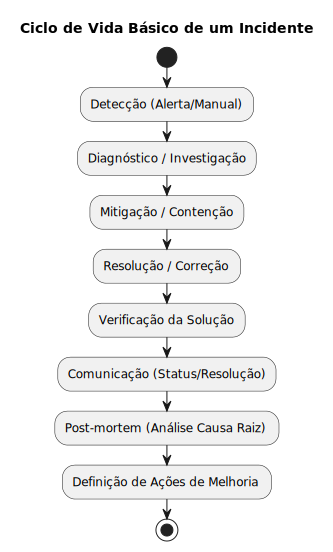
\includegraphics[width=0.9\textwidth]{../assets/diagrama-ciclo-incidente.pdf}
    \caption{Ciclo de Vida Básico de um Incidente}
    \label{fig:ciclo-incidente}
\end{figure}

\begin{itemize}
    \item \textbf{Redução de MTTD (Mean Time To Detect):}
        \begin{itemize}
            \item \textbf{Alertas Acionáveis:} Garantir que os alertas configurados (baseados em SLOs e sintomas) sejam claros, relevantes e direcionem para a possível causa ou impacto. Evitar ruído excessivo de alertas não acionáveis.
            \item \textbf{Dashboards Consolidados (Grafana):} Manter dashboards que mostrem rapidamente a saúde dos serviços principais, o status dos SLOs e métricas chave, facilitando a identificação visual de anomalias.
            \item \textbf{Correlação:} Utilizar as ferramentas de observabilidade (Grafana com Loki/Jaeger/Prometheus) para correlacionar rapidamente métricas, logs e traces durante a investigação inicial.
        \end{itemize}
    \item \textbf{Redução de MTTR (Mean Time To Recover):}
        \begin{itemize}
            \item \textbf{Runbooks/Playbooks:} Documentar procedimentos passo-a-passo para diagnosticar e mitigar incidentes comuns ou alertas específicos. Devem ser mantidos atualizados e facilmente acessíveis.
            \item \textbf{Escalas de Plantão (On-Call):} Definir escalas de plantão claras, com responsabilidades bem definidas e ferramentas adequadas (PagerDuty/Opsgenie) para notificação e escalonamento.
            \item \textbf{Ferramentas de Comunicação:} Utilizar canais dedicados em ferramentas de chat (Slack, Teams) para comunicação focada durante um incidente ("War Room" virtual).
            \item \textbf{Automação de Mitigação (Opcional):} Para incidentes muito bem compreendidos, automatizar ações de mitigação (Exemplo: reiniciar um serviço específico, escalar temporariamente um recurso) via scripts ou ferramentas de automação.
            \item \textbf{Acesso e Permissões:} Garantir que a equipe on-call tenha o acesso necessário e seguro para investigar e aplicar correções nos ambientes.
            \item \textbf{Cultura de Post-mortems "Blameless":}
                \begin{itemize}
                    \item Realizar análises pós-incidente detalhadas para cada incidente significativo.
                    \item Foco em entender a \textbf{causa raiz sistêmica} (tecnologia, processo, monitoramento) e não em culpar indivíduos.
                    \item Documentar o incidente, a linha do tempo, o impacto, as ações tomadas e, principalmente, as \textbf{ações de acompanhamento} (melhorias no código, infraestrutura, monitoramento, runbooks) para prevenir recorrências.
                \end{itemize}
        \end{itemize}
\end{itemize}

\section{Feedback dos Clientes}
\label{sec:feedback-clientes}

A percepção do cliente é a medida final da confiabilidade. Coletar e agir sobre o feedback do cliente é essencial para complementar os dados técnicos de monitoramento.

\subsection{Canais de Coleta}
\label{subsec:canais-coleta}

\begin{table}[htbp]
    \centering
    \caption{Canais de Coleta de Feedback do Cliente}
    \label{tab:canais-coleta}
    \rowcolors{2}{gray!10}{white}
    % Usar tabularx e booktabs.
    \begin{tabularx}{\textwidth}{lX} % Removido '|'
        \toprule
        \textbf{Canal} & \textbf{Descrição / Exemplo} \\
        \midrule
        Pesquisas In-App/Web & Perguntas curtas sobre a experiência após ações chave (reserva, busca). \\
        Formulários de Contato/Suporte & Canal direto para reportar problemas ou dificuldades específicas. \\
        Análise de Chamados de Suporte & Categorizar e analisar os motivos dos contatos com a equipe de suporte. \\
        Monitoramento de Redes Sociais/Avaliação & Acompanhar menções à VOEBEM em plataformas públicas (Twitter, Reclame Aqui). \\
        Pesquisas de Satisfação (NPS/CSAT) & Medir a satisfação geral e a probabilidade de recomendação periodicamente. \\
        \bottomrule
    \end{tabularx}
\end{table}

\subsection{Processamento e Ação}
\label{subsec:processamento-feedback}

\textbf{Fluxo Básico de Tratamento de Feedback:}

\begin{figure}[htbp]
    \centering
    % Reduzindo a largura da imagem
    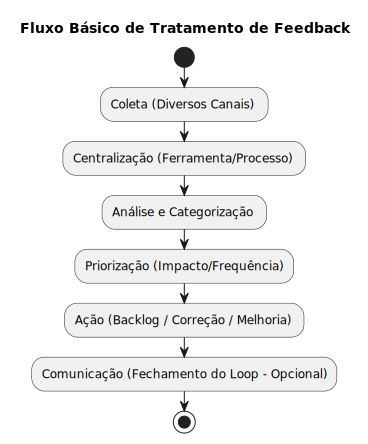
\includegraphics[width=0.9\textwidth]{../assets/diagrama-fluxo-feedback.pdf}
    \caption{Fluxo Básico de Tratamento de Feedback}
    \label{fig:fluxo-feedback}
\end{figure}

\begin{itemize}
    \item \textbf{Centralização:} Agregar o feedback de diferentes canais em uma ferramenta ou processo unificado (Exemplo: um quadro Kanban, uma ferramenta de gestão de feedback).
    \item \textbf{Análise e Categorização:} Identificar temas recorrentes, problemas específicos, sugestões de melhoria. Correlacionar reclamações (Exemplo: lentidão) com dados de monitoramento técnico.
    \item \textbf{Priorização:} Avaliar o impacto e a frequência dos problemas reportados pelos clientes.
    \item \textbf{Integração com Backlog:} Transformar feedback acionável em itens de trabalho (bugs, melhorias) para as equipes de desenvolvimento e SRE.
    \item \textbf{Refinamento de SLIs/SLOs:} Usar o feedback para validar se os SLIs/SLOs atuais refletem a experiência real do usuário ou se novos indicadores são necessários (Exemplo: sucesso na conclusão do fluxo de reserva ponta-a-ponta).
    \item \textbf{Comunicação (Fechamento do Loop):} Informar aos clientes (quando apropriado e possível) sobre as ações tomadas com base em seus feedbacks, demonstrando que a empresa ouve e age.
\end{itemize}

% --- Final do Arquivo ---

% ----------------------------------------------------------
% ELEMENTOS PÓS-TEXTUAIS
% ----------------------------------------------------------
\postextual% Garantido sem espaço

% ----------------------------------------------------------
% Anexos
% ----------------------------------------------------------
\begin{anexos}
% ----------------------------------------------------------
% Anexo A
% ----------------------------------------------------------
\chapter*{Anexo A - Esquema Entidade-Relacionamento (ER) e DBML}
\addcontentsline{toc}{chapter}{Anexo A - Esquema Entidade-Relacionamento (ER) e DBML}
\label{anexo:er-dbml}

Este anexo descreve a estrutura do banco de dados relacional proposto para o sistema VOEBEM, mostrando as entidades principais, seus atributos e os relacionamentos entre elas.

\section*{Diagrama ER}

\begin{figure}[htbp]
    \centering
    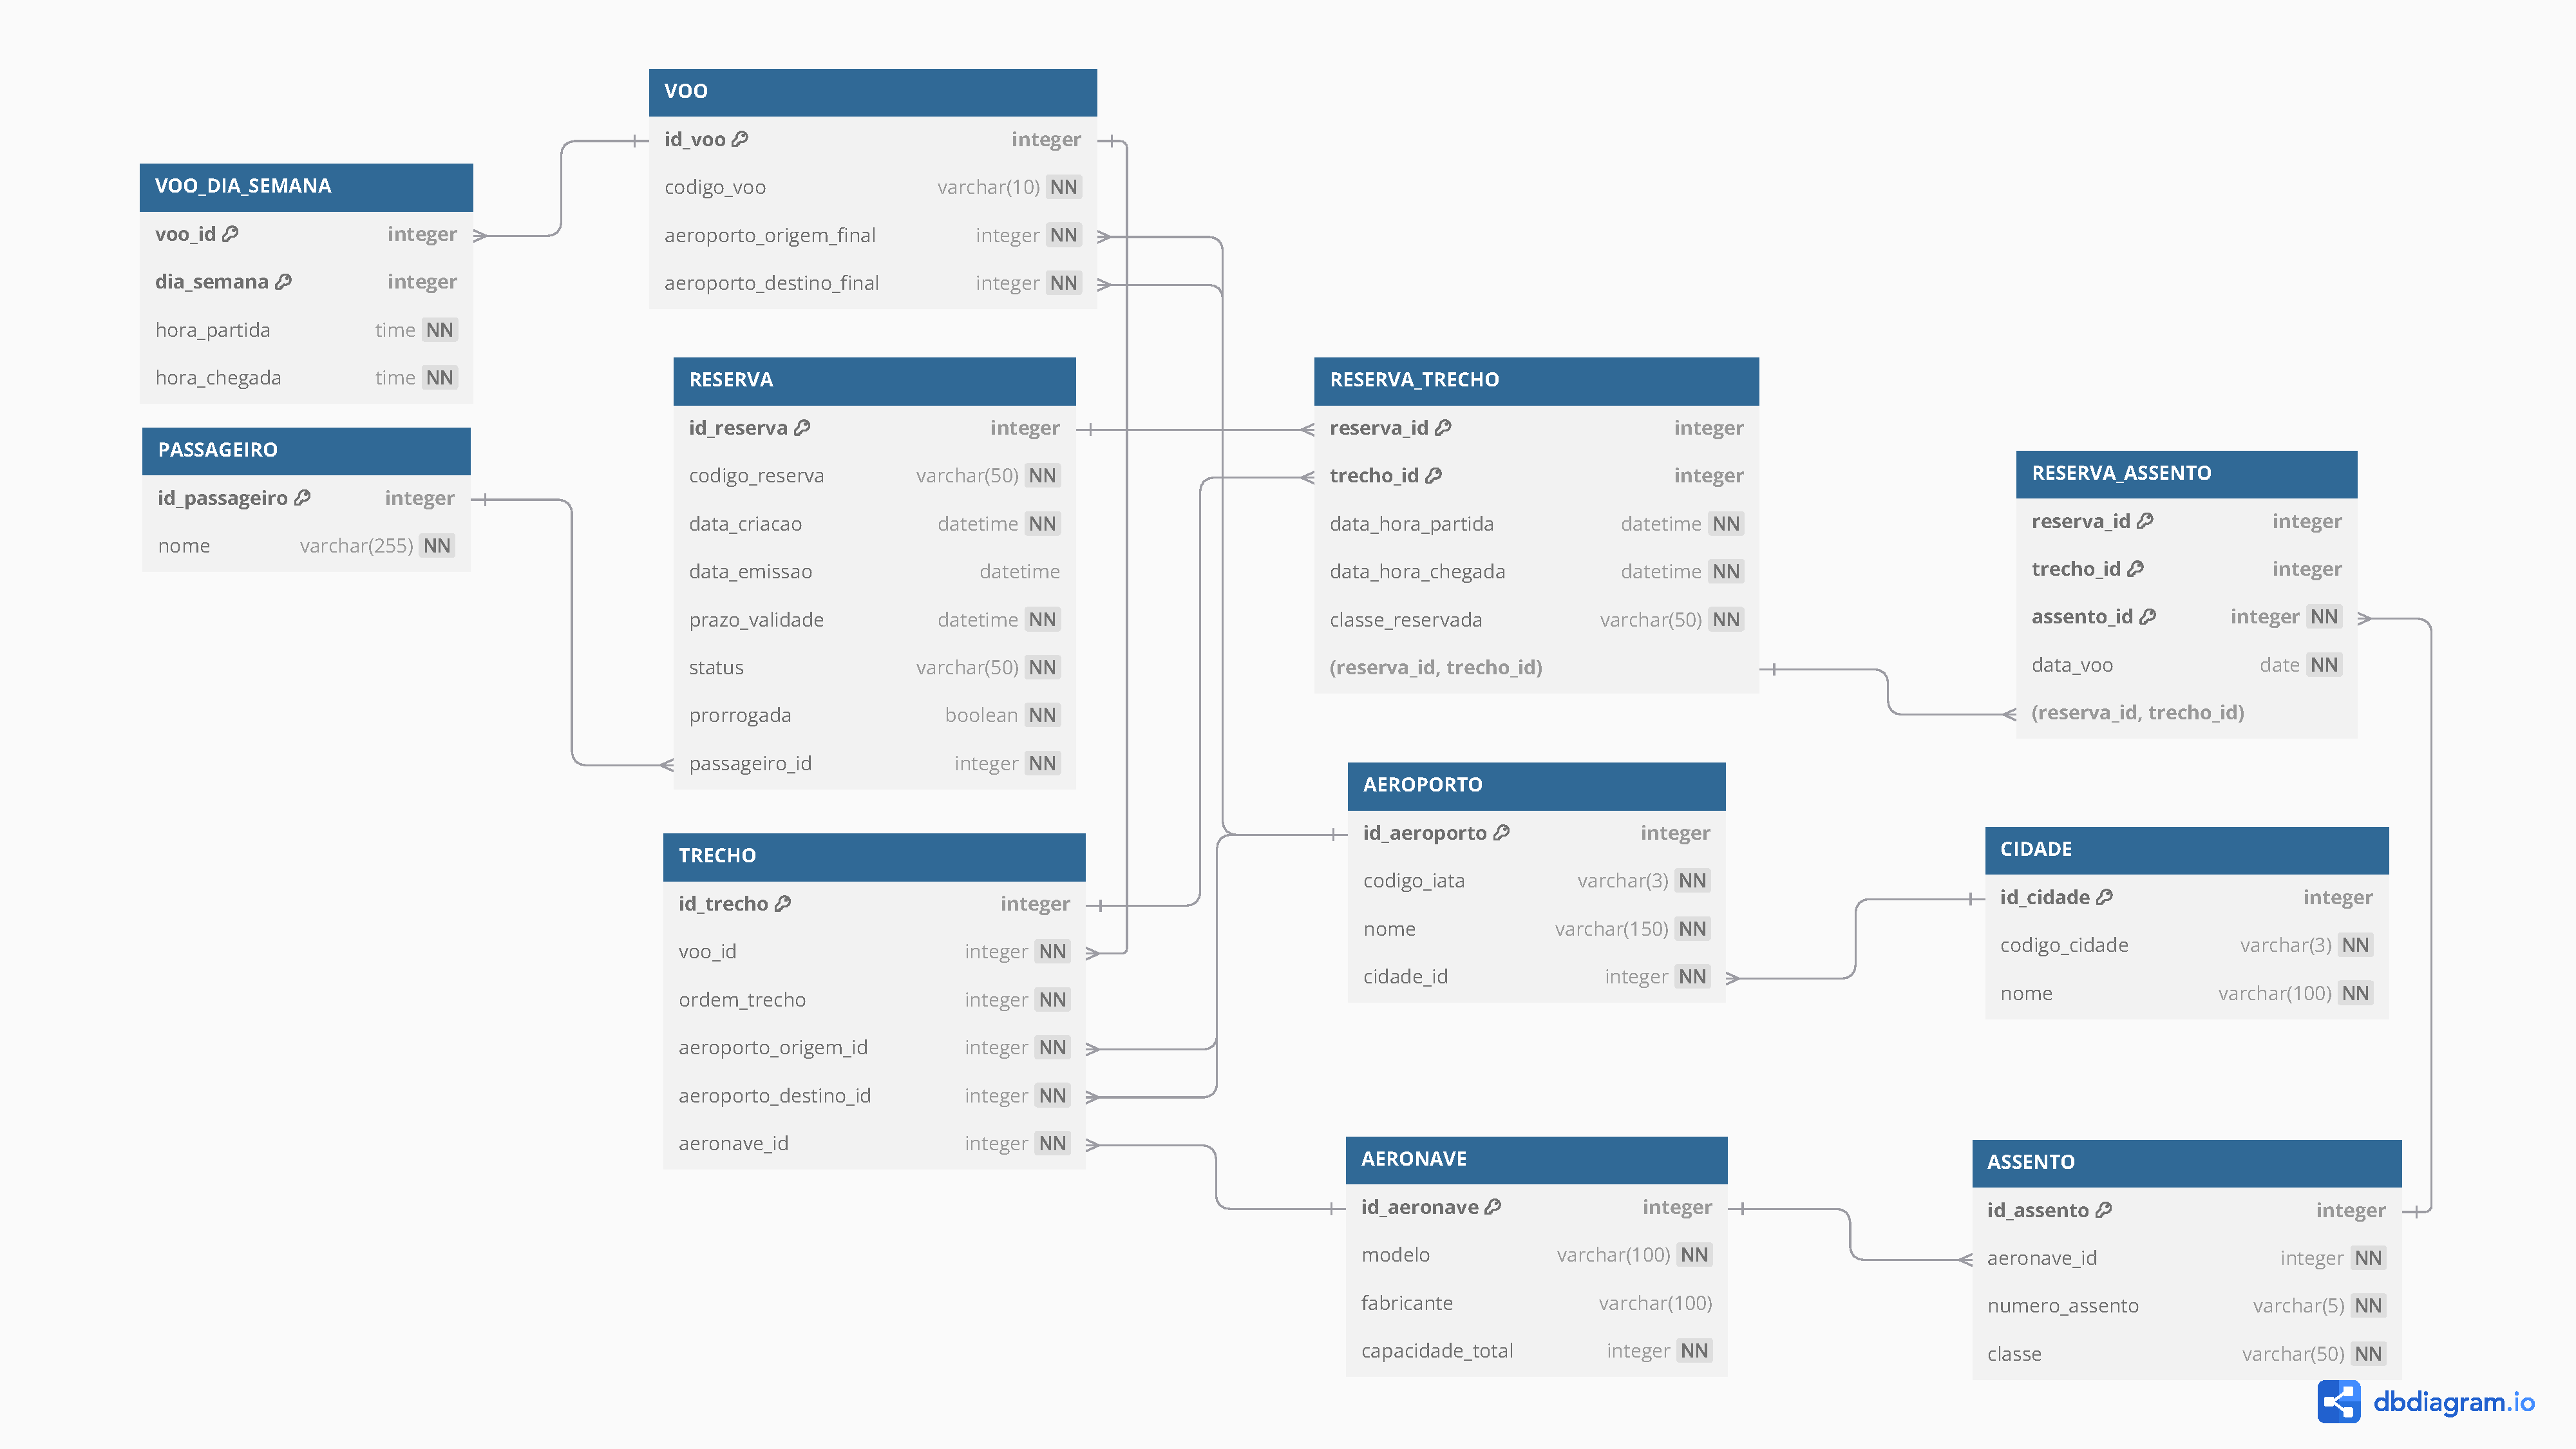
\includegraphics[width=1.4\textwidth, angle=90]{../assets/er-diagram-voebem.pdf}
    \caption{Diagrama ER - Sistema VOEBEM}
    \label{fig:diagrama-er}
\end{figure}

\textit{(Nota: O diagrama acima representa visualmente o esquema definido abaixo.)}

\section*{Descrição das Entidades e Relacionamentos}

\subsection*{Entidades}

\subsubsection*{PASSAGEIRO}
Representa uma pessoa que faz uma reserva.
\begin{itemize}
    \item \texttt{id\_passageiro} (INTEGER): Chave primária, auto-incremento.
    \item \texttt{nome} (VARCHAR): Nome do passageiro, não nulo.
\end{itemize}

\subsubsection*{RESERVA}
Representa uma reserva feita por um passageiro para um ou mais trechos de voo.
\begin{itemize}
    \item \texttt{id\_reserva} (INTEGER): Chave primária, auto-incremento.
    \item \texttt{codigo\_reserva} (VARCHAR): Código único da reserva, não nulo.
    \item \texttt{data\_criacao} (DATETIME): Data e hora de criação da reserva, não nulo (padrão: data/hora atual).
    \item \texttt{data\_emissao} (DATETIME): Data e hora de emissão (confirmação) da reserva, pode ser nulo.
    \item \texttt{prazo\_validade} (DATETIME): Prazo limite para confirmação da reserva, não nulo.
    \item \texttt{status} (VARCHAR): Status atual da reserva (Ex: Pendente, Confirmada, Cancelada, Emitida), não nulo.
    \item \texttt{prorrogada} (BOOLEAN): Indica se o prazo de validade foi prorrogado, não nulo (padrão: false).
    \item \texttt{passageiro\_id} (INTEGER): Chave estrangeira referenciando o passageiro que fez a reserva, não nulo.
    \item \texttt{fonte\_reserva} (VARCHAR): Origem da reserva (Ex: Interno, Web, GDS\_Amadeus), pode ser nulo.
    \item \texttt{id\_externo\_reserva} (VARCHAR): ID da reserva no sistema externo (Ex: GDS PNR), pode ser nulo.
    \item \texttt{id\_transacao\_pagamento} (VARCHAR): ID da transação no sistema de pagamento, pode ser nulo.
    \item \texttt{status\_pagamento} (VARCHAR): Status do pagamento (Ex: Pendente, Aprovado, Falhou), pode ser nulo.
    \item \texttt{valor\_pago} (DECIMAL): Valor efetivamente pago pela reserva, pode ser nulo.
\end{itemize}

\subsubsection*{VOO}
Representa um voo como uma sequência de trechos, com origem e destino finais.
\begin{itemize}
    \item \texttt{id\_voo} (INTEGER): Chave primária, auto-incremento.
    \item \texttt{codigo\_voo} (VARCHAR): Código único do voo, não nulo.
    \item \texttt{aeroporto\_origem\_final} (INTEGER): Chave estrangeira referenciando o aeroporto de origem final do voo, não nulo.
    \item \texttt{aeroporto\_destino\_final} (INTEGER): Chave estrangeira referenciando o aeroporto de destino final do voo, não nulo.
\end{itemize}

\subsubsection*{TRECHO}
Representa um segmento individual de um voo, conectando dois aeroportos com uma aeronave específica.
\begin{itemize}
    \item \texttt{id\_trecho} (INTEGER): Chave primária, auto-incremento.
    \item \texttt{voo\_id} (INTEGER): Chave estrangeira referenciando o voo ao qual este trecho pertence, não nulo.
    \item \texttt{ordem\_trecho} (INTEGER): Ordem do trecho dentro do voo, não nulo (compõe chave única com \texttt{voo\_id}).
    \item \texttt{aeroporto\_origem\_id} (INTEGER): Chave estrangeira referenciando o aeroporto de origem deste trecho, não nulo.
    \item \texttt{aeroporto\_destino\_id} (INTEGER): Chave estrangeira referenciando o aeroporto de destino deste trecho, não nulo.
    \item \texttt{aeronave\_id} (INTEGER): Chave estrangeira referenciando a aeronave usada neste trecho, não nulo.
\end{itemize}

\subsubsection*{VOO\_DIA\_SEMANA}
Indica em quais dias da semana um voo específico opera e seus horários.
\begin{itemize}
    \item \texttt{voo\_id} (INTEGER): Chave primária composta, chave estrangeira referenciando o voo.
    \item \texttt{dia\_semana} (INTEGER): Chave primária composta, dia da semana (0=Domingo, 6=Sábado).
    \item \texttt{hora\_partida} (TIME): Hora de partida neste dia da semana, não nulo.
    \item \texttt{hora\_chegada} (TIME): Hora de chegada neste dia da semana, não nulo.
\end{itemize}

\subsubsection*{CIDADE}
Representa uma cidade.
\begin{itemize}
    \item \texttt{id\_cidade} (INTEGER): Chave primária, auto-incremento.
    \item \texttt{codigo\_cidade} (VARCHAR): Código único da cidade (Ex: SAO), não nulo.
    \item \texttt{nome} (VARCHAR): Nome da cidade, não nulo.
\end{itemize}

\subsubsection*{AEROPORTO}
Representa um aeroporto.
\begin{itemize}
    \item \texttt{id\_aeroporto} (INTEGER): Chave primária, auto-incremento.
    \item \texttt{codigo\_iata} (VARCHAR): Código IATA único do aeroporto (Ex: GRU), não nulo.
    \item \texttt{nome} (VARCHAR): Nome do aeroporto, não nulo.
    \item \texttt{cidade\_id} (INTEGER): Chave estrangeira referenciando a cidade onde o aeroporto está localizado, não nulo.
\end{itemize}

\subsubsection*{AERONAVE}
Representa uma aeronave.
\begin{itemize}
    \item \texttt{id\_aeronave} (INTEGER): Chave primária, auto-incremento.
    \item \texttt{modelo} (VARCHAR): Modelo da aeronave, não nulo.
    \item \texttt{fabricante} (VARCHAR): Fabricante da aeronave.
    \item \texttt{capacidade\_total} (INTEGER): Capacidade total de passageiros da aeronave, não nulo.
\end{itemize}

\subsubsection*{ASSENTO}
Representa um assento individual em uma aeronave.
\begin{itemize}
    \item \texttt{id\_assento} (INTEGER): Chave primária, auto-incremento.
    \item \texttt{aeronave\_id} (INTEGER): Chave estrangeira referenciando a aeronave à qual o assento pertence, não nulo.
    \item \texttt{numero\_assento} (VARCHAR): Número/identificação do assento (compõe chave única com \texttt{aeronave\_id}), não nulo.
    \item \texttt{classe} (VARCHAR): Classe do assento (Ex: Econômica, Executiva), não nulo.
\end{itemize}

\subsubsection*{RESERVA\_TRECHO}
Tabela associativa que liga uma RESERVA a um TRECHO específico que faz parte dessa reserva.
\begin{itemize}
    \item \texttt{reserva\_id} (INTEGER): Parte da chave primária composta, chave estrangeira referenciando a RESERVA.
    \item \texttt{trecho\_id} (INTEGER): Parte da chave primária composta, chave estrangeira referenciando o TRECHO.
    \item \texttt{data\_hora\_partida} (DATETIME): Data e hora de partida programada para este trecho na reserva, não nulo.
    \item \texttt{data\_hora\_chegada} (DATETIME): Data e hora de chegada programada para este trecho na reserva, não nulo.
    \item \texttt{classe\_reservada} (VARCHAR): Classe em que o assento foi reservado para este trecho, não nulo.
\end{itemize}

\subsubsection*{RESERVA\_ASSENTO}
Tabela associativa que liga um \texttt{RESERVA\_TRECHO} a um \texttt{ASSENTO} específico reservado para uma data de voo particular.
\begin{itemize}
    \item \texttt{reserva\_id} (INTEGER): Parte da chave primária composta, chave estrangeira referenciando \texttt{RESERVA\_TRECHO}.
    \item \texttt{trecho\_id} (INTEGER): Parte da chave primária composta, chave estrangeira referenciando \texttt{RESERVA\_TRECHO}.
    \item \texttt{assento\_id} (INTEGER): Parte da chave primária composta, chave estrangeira referenciando o ASSENTO, não nulo.
    \item \texttt{data\_voo} (DATE): Data específica em que este trecho do voo está sendo reservado para este assento (compõe chave única com \texttt{assento\_id} e \texttt{trecho\_id}), não nulo.
    \item \texttt{status\_checkin} (VARCHAR): Status do check-in para este assento/trecho (Ex: Pendente, Realizado), pode ser nulo.
\end{itemize}

\subsection*{Relacionamentos}
\begin{description}
    \item[\texttt{PASSAGEIRO} -- \texttt{RESERVA}:] \texttt{PASSAGEIRO} \textbf{faz} uma ou mais (\texttt{o\{\}}) \texttt{RESERVA}s.
    \item[\texttt{RESERVA} -- \texttt{RESERVA\_TRECHO}:] \texttt{RESERVA} \textbf{contem\_trecho} um ou mais (\texttt{o\{\}}) \texttt{RESERVA\_TRECHO}s.
    \item[\texttt{TRECHO} -- \texttt{RESERVA\_TRECHO}:] \texttt{TRECHO} \textbf{eh\_reservado\_em} zero ou mais (\texttt{o\{\}}) \texttt{RESERVA\_TRECHO}s.
    \item[\texttt{VOO} -- \texttt{TRECHO}:] \texttt{VOO} \textbf{composto\_por} um ou mais (\texttt{o\{\}}) \texttt{TRECHO}s.
    \item[\texttt{AEROPORTO} -- \texttt{TRECHO} (Origem):] \texttt{AEROPORTO} pode ser a \textbf{origem\_de} zero ou mais (\texttt{o\{\}}) \texttt{TRECHO}s.
    \item[\texttt{AEROPORTO} -- \texttt{TRECHO} (Destino):] \texttt{AEROPORTO} pode ser o \textbf{destino\_de} zero ou mais (\texttt{o\{\}}) \texttt{TRECHO}s.
    \item[\texttt{AERONAVE} -- \texttt{TRECHO}:] \texttt{AERONAVE} é \textbf{usado\_em} zero ou mais (\texttt{o\{\}}) \texttt{TRECHO}s.
    \item[\texttt{VOO} -- \texttt{VOO\_DIA\_SEMANA}:] \texttt{VOO} \textbf{opera\_em} um ou mais (\texttt{o\{\}}) \texttt{VOO\_DIA\_SEMANA}s.
    \item[\texttt{CIDADE} -- \texttt{AEROPORTO}:] \texttt{CIDADE} é \textbf{localizado\_em} zero ou mais (\texttt{o\{\}}) \texttt{AEROPORTO}s.
    \item[\texttt{AERONAVE} -- \texttt{ASSENTO}:] \texttt{AERONAVE} \textbf{possui} um ou mais (\texttt{o\{\}}) \texttt{ASSENTO}s.
    \item[\texttt{AEROPORTO} -- \texttt{VOO} (Origem Final):] \texttt{AEROPORTO} pode ser a \textbf{origem\_final\_em} zero ou mais (\texttt{o\{\}}) \texttt{VOO}s.
    \item[\texttt{AEROPORTO} -- \texttt{VOO} (Destino Final):] \texttt{AEROPORTO} pode ser o \textbf{destino\_final\_em} zero ou mais (\texttt{o\{\}}) \texttt{VOO}s.
    \item[\texttt{RESERVA\_TRECHO} -- \texttt{RESERVA\_ASSENTO}:] \texttt{RESERVA\_TRECHO} tem um \textbf{assento\_reservado\_para} zero ou mais (\texttt{o\{\}}) \texttt{RESERVA\_ASSENTO}s.
    \item[\texttt{ASSENTO} -- \texttt{RESERVA\_ASSENTO}:] \texttt{ASSENTO} é \textbf{reservado\_em} zero ou mais (\texttt{o\{\}}) \texttt{RESERVA\_ASSENTO}s.
\end{description}

\section*{Esquema DBML}

Abaixo está o esquema do banco de dados definido usando a sintaxe DBML (Database Markup Language). Este esquema é uma representação textual do diagrama ER, facilitando a criação e manutenção do banco de dados.

\begin{lstlisting}[language={}, % Nenhuma linguagem específica definida para DBML no listings
    basicstyle=\footnotesize\ttfamily, % Fonte monoespaçada pequena
    breaklines=true, % Quebra linhas longas automaticamente
    caption={Esquema DBML - Sistema VOEBEM},
    label={lst:dbml-schema},
    showstringspaces=false, % Não mostra espaços em strings de forma especial
    tabsize=2, % Define o tamanho da tabulação
    frame=single, % Adiciona uma moldura simples
    numbers=left, % Adiciona numeração de linhas à esquerda
    numberstyle=\tiny\color{gray}, % Estilo da numeração de linhas
    % --- Correções para caracteres especiais --- 
    literate={_}{{\_}}1 % Trata underscore como texto literal
             {`}{{\texttt{\`}}}1, % Trata backtick como texto literal (usando texttt)
             % Aspas simples (') parecem ok, pois já estão escapadas nas notas
             % Maior que (>) em Refs parece ok por padrão
    % -------------------------------------------
    % Estilos opcionais (podem ser removidos se causarem problemas)
    keywordstyle=\color{blue}, 
    commentstyle=\color{green!60!black}, 
    stringstyle=\color{purple}
]
Table PASSAGEIRO {
  id_passageiro integer [pk, increment]
  nome varchar(255) [not null]
}

Table RESERVA {
  id_reserva integer [pk, increment]
  codigo_reserva varchar(50) [unique, not null]
  data_criacao datetime [default: `now()`, not null]
  data_emissao datetime [null]
  prazo_validade datetime [not null]
  status varchar(50) [not null, note: 'Pendente, Confirmada, Cancelada, Expirada']
  prorrogada boolean [default: false, not null]
  passageiro_id integer [not null]

  Indexes {
    (codigo_reserva)
  }
}

Table VOO {
  id_voo integer [pk, increment]
  codigo_voo varchar(10) [unique, not null]
  aeroporto_origem_final integer [not null]
  aeroporto_destino_final integer [not null]
  Indexes {
    (codigo_voo)
  }
}

Table TRECHO {
  id_trecho integer [pk, increment]
  voo_id integer [not null]
  ordem_trecho integer [not null, note: 'Sequência do trecho dentro do voo (1, 2, ...)' ]
  aeroporto_origem_id integer [not null]
  aeroporto_destino_id integer [not null]
  aeronave_id integer [not null, note: 'Aeronave planejada para este trecho']

  Indexes {
    (voo_id, ordem_trecho) [unique]
  }
}

Table VOO_DIA_SEMANA {
  voo_id integer [pk]
  dia_semana integer [pk, note: '0=Domingo, 1=Segunda,..., 6=Sábado']
  hora_partida time [not null]
  hora_chegada time [not null]
}

Table CIDADE {
  id_cidade integer [pk, increment]
  codigo_cidade varchar(3) [unique, not null, note: 'Ex: SAO, RIO']
  nome varchar(100) [not null]

  Indexes {
    (codigo_cidade)
  }
}

Table AEROPORTO {
  id_aeroporto integer [pk, increment]
  codigo_iata varchar(3) [unique, not null, note: 'Ex: GRU, GIG, POA']
  nome varchar(150) [not null]
  cidade_id integer [not null]

  Indexes {
    (codigo_iata)
  }
}

Table AERONAVE {
  id_aeronave integer [pk, increment]
  modelo varchar(100) [not null]
  fabricante varchar(100)
  capacidade_total integer [not null]
}

Table ASSENTO {
  id_assento integer [pk, increment]
  aeronave_id integer [not null]
  numero_assento varchar(5) [not null, note: 'Ex: 1A, 20F']
  classe varchar(50) [not null, note: 'Econômica, Executiva, Primeira Classe']

  Indexes {
    (aeronave_id, numero_assento) [unique]
  }
}

Table RESERVA_TRECHO {
  reserva_id integer [pk]
  trecho_id integer [pk]
  data_hora_partida datetime [not null, note: 'Data e hora exatas da partida deste trecho para esta reserva']
  data_hora_chegada datetime [not null, note: 'Data e hora exatas da chegada deste trecho para esta reserva']
  classe_reservada varchar(50) [not null, note: 'Classe específica reservada para este trecho (pode ser diferente da classe do assento)']
}

Table RESERVA_ASSENTO {
  reserva_id integer [pk]
  trecho_id integer [pk]
  assento_id integer [pk, not null]
  data_voo date [not null, note: 'Data específica do voo para esta reserva de assento']

  Indexes {
    (assento_id, trecho_id, data_voo) [unique]
  }
}

Ref: RESERVA.passageiro_id > PASSAGEIRO.id_passageiro
Ref: RESERVA_TRECHO.reserva_id > RESERVA.id_reserva
Ref: RESERVA_TRECHO.trecho_id > TRECHO.id_trecho
Ref: TRECHO.voo_id > VOO.id_voo
Ref: TRECHO.aeroporto_origem_id > AEROPORTO.id_aeroporto
Ref: TRECHO.aeroporto_destino_id > AEROPORTO.id_aeroporto
Ref: TRECHO.aeronave_id > AERONAVE.id_aeronave
Ref: VOO_DIA_SEMANA.voo_id > VOO.id_voo
Ref: AEROPORTO.cidade_id > CIDADE.id_cidade
Ref: ASSENTO.aeronave_id > AERONAVE.id_aeronave
Ref: VOO.aeroporto_origem_final > AEROPORTO.id_aeroporto
Ref: VOO.aeroporto_destino_final > AEROPORTO.id_aeroporto
Ref: RESERVA_ASSENTO.(reserva_id, trecho_id) > RESERVA_TRECHO.(reserva_id, trecho_id)
Ref: RESERVA_ASSENTO.assento_id > ASSENTO.id_assento
\end{lstlisting}

% --- Final do Arquivo ---

% ---
% Bibliografia
% ---
\nocite{*} % Inclui todas as referências do .bib, mesmo sem \cite
\bibliography{referencias} % Cria um arquivo chamado referencias.bib para suas referências
\bibliographystyle{abntex2-alf} % Define o estilo da bibliografia (ABNT alfabético)
% ---

%---------------------------------------------------------------------
% INDICE REMISSIVO
%---------------------------------------------------------------------
% \printindex % Descomente se você usar um índice remissivo com \makeindex

\end{document}
